\lecture{Tue. 9/18/12}

The course website is
\url{http://math.mit.edu/\~tfei}. The first homework is due on Tuesday of next week.

Recall that to differentiate a vector field in the directino of another, we needed to identify different vector spaces; one way to do so was with the Lie derivative. Another way is to equip the manifold with extra structure, a Riemannian connection. We'll cover this today, and show how from an affine connection we can also define the covariant derivative, which is a generalization of differentiating a vector field along a curve.

\subsection{Affine connection}

For $M$ a smooth $n$-dimensional manifold, let $\X(M)$ be the set of vector fields on $M$.

\begin{df}
An \textbf{affine connection} on $M$ is a function $\nabla:\X(M)\times \X(M)\to \X(M)$ with the following properties.
\begin{enumerate}
\item
$\nabla_Z(X+fY)=\nabla_ZX+Z(f)Y+f\nabla_ZY$
\item
$\nabla_{X+fY}Z=\nabla_XZ+f\nabla_YZ$.
\end{enumerate}
\end{df}
\begin{ex}\llabel{ex:Rn-ac}
The affine connection on $\R^n$ is given as follows. Suppose $X=\sui a_i\pd{}{x_i}$ and $Y=\sui b_i\pd{}{x_i}$. Then
\[
\nabla_XY=\suij a_{i}\pd{b_j}{x_i}\pd{}{x_j};
\]
i.e. the affine connection is just differentiating $(b_1,\ldots, b_n)$ in the direction of $X$.
%$X,Y,Z$ vector fields on $\R^u$ vector valued functions. $Y(X)=dX(Y)$.
\end{ex}
%$X,Y,Z\in X(M)$. $f:M\to \R$ smooth function on $M$.

Note an affine connection basically tells us how to differentiate one vector field with respect to another.

\begin{df}
Suppose $M^n$ is a smooth manifold, $\nabla$ is a connection, and $c:I\to M$ is an interval. A \textbf{vector field} $V$ along the curve $c$ is a function such that for $t\in I$, $V(t)\in T_{c(t)}M$ and $t\mapsto V(t)$ is smooth. 
\end{df}
Note $V(t)$ is not necessarily the restriction of a vector field on $M$, but is a vector field along the curve. For instance, the velocity field along the following self-intersecting curve is a vector field along the curve that is not the restriction of a vector field on $\R^2$. This is becaue at the point of intersection, there are two vectors.
%only bad case.

\begin{center}
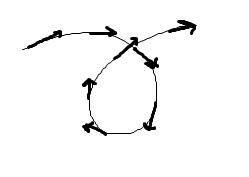
\includegraphics{5-1}
\end{center}

\begin{df}\llabel{df:covar-der}
Let $c:I\to M$ be a smooth curve and $\nabla$ be a connection. There is a unique operation $\fc{D}{\partial t}$ called the \textbf{covariant derivative} along the curve (sending vector fields along the curve to vector fields along the curve) with the following properties.
\begin{enumerate}
\item (Additivity and Leibniz rule)
If $V,W$ are vector fields along the curve and $f:I\to \R$, then
\[
\fc{D}{\partial t}(V+fW)= \fc{D}{\partial t}V+f\fc{D}{\partial t}W+f'W.
\]
\item If $X\in \X(M)$ then
\[
\fc{D}{\partial t}X=\nabla_{c'}X.
\]
\end{enumerate}
\end{df}
%convention
%at the field, if vector field on manifold, capital X,Y,Z. vector field on curve V, W
Think of this as the derivative of a vector field along the curve.

\begin{pr}
Suppose $\nabla$ is a connection, $X,Y,Z\in \X(M)$, and $p\in M$. If $X(p)=Y(p)$, then 
\[
(\nabla_X Z)(p)=(\nabla_Y Z)(p).
\]
\end{pr}
Consider the canonical connection on $\R^n$ as in Example~\ref{ex:Rn-ac}, %The model for a connection: vector field is vector-valued function. The canonical connection on $\R^n$ is 
$\nabla_YX%=Y(X)
=dX(Y)$. %; it has the required properties.
If you evaluate at $p$, it depends on what $X$ is close to $p$, but as for $Y$, it only depends on the value of $Y$ at $p$.

\begin{proof}
Use the fact
\[
\nabla_{X+fY}Z=\nabla_XZ+f\nabla_YZ.
\]
Suppose we have local coordinates $(x_1,\ldots, x_n)$ on $M$. Write $X=a_i\pd{}{x_i}$ and $Y=b_i\pd{}{x_i}$ (repeated indices are summed) where $a_i$ and $b_i$ are smooth functions on $M$. Now by linearity in the subscript,
\[
\nabla_XZ=\nabla_{a_i\pd{}{x_i}}Z=a_i \nabla_{\pd{}{x_i}}Z,
\]
and the same is true for $Y$. Evaluating at $p$, we get that they are equal at $p$.
\end{proof}
\begin{df}
Given local coordinates on a manifold with an affine connection, define the \textbf{christoffel symbols} as the constants $\Ga_{ij}^k$ that make the following true:
\[
\nabla_{\pd{}{x_i}}{\pd{}{x_j}}=:\Ga_{ij}^k \pd{}{x_k}.
\]
\end{df}

If we have two vector fields $X$ and $Y$, writing $X=a_i\pd{}{x_i}$ and $Y=b_j\pd{}{x_j}$, then
\bal
\nabla_X Y&=\nabla_{a_i\pd{}{x_i}}\pa{b_j\pd{}{x_j}}\\
&=a_i\nabla_{\pd{}{x_i}}\pa{b_j\pd{}{x_j}}\\
&=a_ib_j\nabla_{\pd{}{x_i}} \pd{}{x_j}+a_i\pd{}{x_i}(b_j)\pd{}{x_j}\\
&=a_ib_j \Ga_{ij}^k \pd{}{x_k}+a_i\pd{}{x_i}(b_j)\pd{}{x_j}.
\end{align*}
Note in the case of $\R^n$ that $\Ga_{ij}^k=0$ for all $i, j, k$.

\subsection{Covariant derivative}
\begin{proof}[Proof of existence and uniqueness of Definition~\ref{df:covar-der}]
Given an affine connection $\nabla$, $c:I\to M$, and $\nabla$, $V$, $W$ vector fields along $c$, $X\in \X(M)$, $\fc{D}{\partial t}$ is another vector field along $c$.

From the condition $\cvd X=\nabla_{c'} X$, if we want to know value at some point, than we just need to know the velocity at that point. %Extend it to any vector field, value will be the same.

Given $V=a_i\pd{}{x_i}$, $a_i:I\to \R$, we must have 
\beq{eq:965-4-1}
\cvd V=a_i'\pd{}{x_i}+a_i\cvd \pa{\pd{}{x_i}}=a_i'\pd{}{x_i}+a_i\nabla_{c'} \pd{}{x_i}
\eeq
where in the last equality we used that $\pd{}{x_i}$ is a global vector field.
We've shown that $\cvd$ only defined one way, by~\eqref{eq:965-4-1}. Conversely, if $\cvd$ is defined by this, it is easy to see that it has the right properties.
\end{proof}


\begin{df}
Given a manifold $M$, a curve $c:I\to M$, an affine connection $\nabla$, and the corresponding covariant derivative $\cvd$,
we say that a vector field $V$ along $c$ is \textbf{parallel} if
\[
\cvd V=0.
\]
\end{df}
Writing $a:I\to \R$, $V=a_i\pd{}{x_i}$, $c'=c_j'\pd{}{x_j}$, we have
\bal
\cvd V&=a_i'\pd{}{x_i}+a_i\nabla_{c'} \pd{}{x_i}\\
&=a_i'\pd{}{x_i} +a_ic_j'\Ga_{ji}^k \pd{}{x_k}.
\end{align*}
To say that $V$ is parallel is just saying 
\bal
0&=a_i'\pd{}{x_i} +a_ic_j'\Ga_{ji}^k \pd{}{x_k}\\
\iff 0&=(a_{\ell}'+a_ic_j'\Ga_{ji}^{\ell})\pd{}{x_k}\\
\iff 0&=a_{\ell}'+a_ic_j'\Ga_{ji}^{\ell}\text{ for all }\ell.
\end{align*}
This is an ODE! Thus, if we prescribe what the $a_i$ are initially, then by existence and uniqueness of solutions to a first-order linear ODE, we have the following proposition.


%\fixme{Figure 2.}
\begin{pr}\llabel{pr:parallel-vf}
Let $c$ be a curve $I=[0,1]\to M$. 
For each value $V(0)\in T_{c(0)}$, there exists a unique vector field $V$ along $c$ that is parallel and initially has this value.

If $V$ and $W$ are parallel, then $V+\la W$ is also parallel.
\end{pr}

\begin{center}
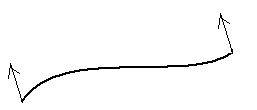
\includegraphics[scale=0.5]{4-2}
\end{center}

\begin{df}
Let $c:I=[0,1]\to M$ be a curve. Define the \textbf{parallel transport} map 
\[
P:T_{c(0)}M\to T_{c(1)}M
\]
as follows. For $v\in T_{c(0)}M$, let $V$ be a parallel vector field along $c$ with $V(0)=v$. Define
\[
P(v)=V(1).
\]
\end{df}
$P$ is a linear map by Proposition~\ref{pr:parallel-vf}.
%Suppose $T_{c(0)}\xra{P}T_{c(1)}M$. $\vartheta\in T_{c(0)} M$, $P(v)=V(1)$. $V(0)=v$, $V$ is parallel. $P$ is a linear map by proposition above. 

%trivial in linear space
\begin{ex}
%How to think about this. 
Take a curve in a plane; think of the plane as a manifold. Take a vector at one end of the curve. What vector on the other end of the curve does it make sense to identify the vector with? The same one!

The vector at the other end does not depend on curve. But, in general, parallel transport depends on the curve. For instance, consider the case of a sphere.

\ig{4-3}{0.5}

In fact, we will see later that the difference is given by the curvature. 
\end{ex}
\cpbox{An affine connection and a curve allows us to identify the  tangent space at one point with the tangent space of another point.\\

It also allows us to differentiate one vector field in the direction of another.}

\vskip0.15in

%Consider a sphere. The identification depends very much on the curve. In fact the difference is given by the curvature. 
In general, without a given curve, we cannot identify tangent spaces at different points without imposing coordinates. If we have a curve, though, we get at least one way to identify those tangent spaces. %, if you have curve. Kind of universal.

Suppose again that we have $M,\nabla,c$, $\cvd(V)$. Suppose for convenience that $c:[0,1]\to M$. Write $V=a_i\pd{}{x_i}$.
Suppose that at $c(0)$, $X_1,\ldots,X_n$ is a basis for $T_{c(0)}$. Then there exists a unique $X_i(t)$ defined as follows:
\[
X_i(t)=P_{c|_{[0,t]}}X_i.
\]
%Note we defined $P:T_{c(0)}M\to T_{c(1)}M$, but we could 
We get $n$ vector fields along the curve. At each point on the curve $c$ that $\{X_i(t)\}_i$ are linearly independent. To see this, note that they are linearly dependent initially, and that by uniqueness in Proposition~\ref{pr:parallel-vf}, parallel translation is symmetric; going forwards and then backwards on the curve gives the identity. If the $X_i(t)$ were linearly dependent at time $t$, we can parallel transport backwards to get a linear dependence relation at time $t=0$, contradiction. %get non-uniqueness of solution.

We can write any vector field as $V=a_iX_i$ where $a_i$ are smooth functions $I\to \R$. Now %formal nonsense
\[
\cvd V=a_i \cvd X_i+a_i'X_i=a_i'X_i
\]
where the first term is 0 because $X_i$ is a parallel basis. Thus we see that the covariant derivative is especially simple.

Recall that given $M$, $p\in M$, a {\it Riemannian metric} is a smoothly varying inner product on the tangent space.

Other structures are interesting, too: Instead of inner product, we could have indefinite (nondegenerate symmetric bilinear) forms. For example, we could consider a Lorentzian. If you study general relativity, then it's all about the Lorentzian metric. Think about a manifold as both space and time; on space we have a Riemannian metric, and on time, we have another bilinear form that is negative definite.

\subsection{Compatibility of metric and connection}
Note that in our study of connections so far, the metric didn't play a role at all. We now bring in the metric. We want the connection to be compatible with the Riemannian metric.
\begin{df}
Let $(M^n,g)$ be a smooth Riemannian manifold and a connection $\nabla$. We say that $g$ is \textbf{compatible} with $\nabla$ if whenever $c:I\to M$ is a curve and $V$ and $W$ are parallel vector fields along $c$, then $g(V,W)$ is constant along $c$. 
%intuitive
\end{df}
If $C:[0,1]\to M$ and $V(0)\perp W(0)$, then $V\perp W$ everywhere along the curve and $|V||W|$ is constant.

\begin{ex}
Take the canonical example $\R^n$, $\nabla$. Let $g=\an{\cdot,\cdot}$ be the usual inner product. Then the connection is compatible with the metric:
The inner product of parallel vector fields is constant along the curve. 
\end{ex}

%riemannian metric, unique connection. Will prove. Prove defn is equiv to more standard about what compat connection is.
%go through most of book, not ch. 10, for certain, ch. 13, then some topics.
Next time we will prove that any Riemannian metric gives rise to a unique connection, and show that our definition of a connection is equivalent to a more standard definition.